\documentclass{report}
\usepackage[utf8]{inputenc}
\usepackage{amsmath}
\usepackage{amsfonts}
\usepackage{hyperref}
\usepackage{tcolorbox}
\usepackage{breqn}
\usepackage{adjustbox}
\usepackage{changepage}
\usepackage{rotating}
\usepackage{algorithm}
\usepackage{algpseudocode}
\usepackage{ntheorem}

% Definition
\newtheorem{definition}{Definition}{\bfseries}{\itshape}
\newtheorem*{definition*}{Definition}{\bfseries}{\itshape}

% Theorem
\newtheorem{theorem}{Theorem}{\bfseries}{\itshape}

% Concept
\newtheorem*{concept}{}{\bfseries}{\itshape}

\title{Analysis of diffusion in AES}
\author{Ana Clara Zoppi Serpa\\ Prof. Dr. Ricardo Dahab \\ Dr. Jorge Nakahara Jr.}
\date{\today}

\begin{document}

% relevance of SR
% relevance of MC
% relevance of SB
% relevance of AK

\maketitle

\tableofcontents

\chapter{Analysis of diffusion in AES}
From \textcolor{red}{Chapters X and Y}, we know that each AES $S$-Box achieves complete diffusion, i.e each output bit depends on all input bits, and that an AES round is composed of the \texttt{SubBytes}, \texttt{ShiftRows}, \texttt{MixColumns} and \texttt{AddRoundKey} steps. Furthermore, before the first round, an \texttt{AddRoundKey} is performed and, in the last round, \texttt{MixColumns} is not present. We also know that there are 3 supported key sizes $n_k$ for AES (128 bits, 192 bits and 256 bits), and that the number of rounds $n_r$ varies according to them. For $n_k = 128$, $n_r = 10$. For $n_k = 192$, $n_r = 12$ and, finally, for $n_k = 256$, $n_r = 14$.

In this Chapter, we analyze plaintext and key diffusion in the AES cipher \cite{AES-FIPS}. We show that complete plaintext diffusion is achieved after 2 rounds for all parameter sets, whilst complete key diffusion is achieved after 2 rounds for $n_k = 128$. For $n_k = 192$ and $n_k = 256$, it is achieved after 3 rounds.

We assume the reader is already familiar with:
\begin{itemize}
    \item the AES cipher \cite{AES-FIPS} and its round transformations
    \item the AES key schedule and how the master key is distributed between $k_0$ and $k_1$ for different parameter sets
    \item the fact that the AES $S$-Box achieves complete diffusion of its 8 input bits (see \textcolor{red}{Chapter X} for an $S$-Box diffusion analysis)
    \item GF($2^8$) arithmetic, more specifically the fact that adding two elements of GF($2^8$) is equivalent to performing their bitwise XOR
    \item the XOR Boolean function
\end{itemize}

\section{Notation}
\begin{itemize}
    \item $x$: AES plaintext
    \item $x_i$: $i$-th byte of AES plaintext
    \item $x_i'$: $i$-th byte of AES round $1$ output
    \item $x_i''$: $i$-th byte of AES round $2$ output
    \item $MC$: the matrix used in the \texttt{MixColumns} transformation
    \item $x_i \rightarrow x_z$: $x_i$ depends on $x_z$
    \item $x_i \rightarrow x_p, x_q, ..., x_z$: $x_i$ depends on variables $x_p, x_q, ..., x_z$
    \item $k_r$: AES subkey used at round $r$
    \item $x^{r, SB}$: AES state after the \texttt{SubBytes} transformation of round $r$ has been performed, $r \geq 1$
    \item $x^{r, SR}$: AES state after the \texttt{ShiftRows} transformation of round $r$ has been performed, $r \geq 1$
    \item $x^{r, MC}$: AES state after the \texttt{MixColumns} transformation of round $r$ has been performed, $r \geq 1$
    \item $x^{r, AK}$: AES state after the \texttt{AddRoundKey} transformation of round $r$ has been performed, $r \geq 0$ (because, before the iterations start, there is one \texttt{AddRoundKey} transformation)
    \item $+$: addition in GF($2^8)$
\end{itemize}

\section{Acronyms}
\begin{itemize}
    \item AES: Advanced Encryption Standard
    \item $S$-Box: Substitution Box
\end{itemize}

\section{AES}
For convenience, AES encryption is presented in Algorithm \ref{alg:aes-encryption}.

\begin{algorithm}[H]
\caption{AES Encryption}
\begin{algorithmic}
\Require $x$ (plaintext), $k_0, k_1, \ldots, k_{n_r}$ (subkeys)
\Ensure $y$ (ciphertext)
\State $x \leftarrow \texttt{AddRoundKey}(x, k_0)$
 \For {$r$ from $1$ to $n_r-1$}
        \State $x \leftarrow$ \texttt{SubBytes}$(x)$
        \State $x \leftarrow$ \texttt{ShiftRows}$(x)$
        \State $x \leftarrow$ \texttt{MixColumns}$(x)$
        \State $x \leftarrow$ \texttt{AddRoundKey}$(x, k_r)$
  \EndFor
\State $x \leftarrow$ \texttt{SubBytes}$(x)$
\State $x \leftarrow$ \texttt{ShiftRows}$(x)$
\State $x \leftarrow$ \texttt{AddRoundKey}$(x, k_{n_r})$
\State $y \leftarrow x$
\State \Return $y$
\end{algorithmic}
\label{alg:aes-encryption}
\end{algorithm}

\section{Plaintext diffusion}
The AES state is commonly represented as a $4\times4$ matrix of bytes

\begin{equation*}
x =
\begin{bmatrix}
x_0 & x_4 & x_8 & x_{12}\\
x_1 & x_5 & x_9 & x_{13}\\
x_2 & x_6 & x_{10} & x_{14}\\
x_3 & x_7 & x_{11} & x_{15}
\end{bmatrix}.
\end{equation*}

For the moment, we restrict our analysis to plaintext diffusion. We assume $k_r = 0$ for all rounds of AES, which implies $x^{0, AK} = x$, since $x_i + 0 = x_i$. In other words, the \texttt{AddRoundKey} step is ignored because we are interested in studying plaintext diffusion.

\subsection{The first \texttt{SubBytes}}

After the \texttt{SubBytes} transformation of the first round, the state is
\begin{equation*}
x^{1, SB} =
\begin{bmatrix}
S(x_0) & S(x_4) & S(x_8) & S(x_{12})\\
S(x_1) & S(x_5) & S(x_9) & S(x_{13})\\
S(x_2) & S(x_6) & S(x_{10}) & S(x_{14})\\
S(x_3) & S(x_7) & S(x_{11}) & S(x_{15})
\end{bmatrix}.
\end{equation*}

From \textcolor{red}{Chapter X}, we know that the application of the $S$-Box ensures complete diffusion on the bit level (each bit of $S(x_i)$ depends on all bits of $x_i$). However, it does not ensure dependence between different bytes, i.e $S(x_1)$ does not depend on $x_0$. Therefore, $S(x_i) \rightarrow x_i$.

\subsection{The first \texttt{ShiftRows}}
The \texttt{ShiftRows} step performs a cyclic permutation in each row of the matrix, thus resulting in
\begin{equation*}
x^{1, SR} =
\begin{bmatrix}
S(x_0) & S(x_4) & S(x_8) & S(x_{12})\\
S(x_5) & S(x_9) & S(x_{13}) & S(x_{1})\\
S(x_{10}) & S(x_{14}) & S(x_{2}) & S(x_{6})\\
S(x_{15}) & S(x_3) & S(x_{7}) & S(x_{11})
\end{bmatrix}.
\end{equation*}

\subsection{The first \texttt{MixColumns}}\label{sec:first-mc}

The \texttt{MixColumns} step is the multiplication of each column of the state by
\begin{equation*}
MC = 
\begin{bmatrix}
2 & 3 & 1 & 1\\
1 & 2 & 3 & 1\\
1 & 1 & 2 & 3\\
3 & 1 & 1 & 2
\end{bmatrix}.
\end{equation*}

The first column of the new state is given by
\begin{equation*}
\begin{bmatrix}
2 & 3 & 1 & 1\\
1 & 2 & 3 & 1\\
1 & 1 & 2 & 3\\
3 & 1 & 1 & 2
\end{bmatrix} \cdot
\begin{bmatrix}
S(x_0) \\
S(x_5) \\
S(x_{10}) \\
S(x_{15}) 
\end{bmatrix} =
\begin{bmatrix}
2S(x_0) + 3S(x_5) + S(x_{10}) + S(x_{15})\\
S(x_0) + 2S(x_5) + 3S(x_{10}) + S(x_{15})\\
S(x_0) + S(x_5) + 2S(x_{10}) + 3S(x_{15})\\
3S(x_0) + S(x_5) + S(x_{10}) + 2S(x_{15})
\end{bmatrix}. 
\end{equation*}

Note that, after $MC$ multiplies a column, each element of the resulting column now depends linearly on the others. This applies to the second, third and fourth new columns as well. Therefore,

\begin{equation*}
x^{1, MC} =
\begin{bmatrix}
x_0' & x_4' & x_8' & x_{12}'\\
x_1' & x_5' & x_9' & x_{13}'\\
x_2' & x_6' & x_{10}' & x_{14}'\\
x_3' & x_7' & x_{11}' & x_{15}'
\end{bmatrix},
\end{equation*}

and the following dependencies between bytes now hold:

\begin{itemize}
    \item each $x_i'\rightarrow x_0, x_5, x_{10}, x_{15}$, for $0 \leq i \leq 3$,
    \item each $x_j'\rightarrow x_4, x_9, x_{14}, x_{3}$, for $4 \leq j \leq 7$,
    \item each $x_l'\rightarrow x_8, x_{13}, x_{2}, x_{7}$, for $8 \leq l \leq 11$,
    \item each $x_m'\rightarrow x_{12}, x_{1}, x_{6}, x_{11}$, for $12 \leq m \leq 15$.
\end{itemize}

The next transformation would be \texttt{AddRoundKey}, but $x^{1, AK} = x^{1, MC}$ because all the subkeys are assumed to be zero. We thus move to the analysis of the second round.

\subsection{The second \texttt{SubBytes}}
Similarly to the first \texttt{SubBytes}, the application of $S$-Boxes ensures that all bits of $S(x_i')$ depend on all bits of $x_i'$, but does not incur dependence between $x_i'$ and $x_j'$ for $i \neq j$.

\subsection{The second \texttt{ShiftRows}}
The rows of the state matrix are cyclically shifted, resulting in
\begin{equation*}
x^{2, SR} =
\begin{bmatrix}
S(x_0') & S(x_4') & S(x_8') & S(x_{12}')\\
S(x_5') & S(x_9') & S(x_{13}') & S(x_{1}')\\
S(x_{10}') & S(x_{14}') & S(x_{2}') & S(x_{6}')\\
S(x_{15}') & S(x_3') & S(x_{7}') & S(x_{11}')
\end{bmatrix}.
\end{equation*}

\subsection{The second \texttt{MixColumns}}\label{sec:second-mc}
Analogously to the first \texttt{MixColumns}, the multiplication by $MC$ causes bytes of the same column to spread their dependence. Therefore,

\begin{equation*}
x^{2, MC} = 
\begin{bmatrix}
x_0'' & x_4'' & x_8'' & x_{12}''\\
x_1'' & x_5'' & x_9'' & x_{13}''\\
x_2'' & x_6'' & x_{10}'' & x_{14}''\\
x_3'' & x_7'' & x_{11}'' & x_{15}''
\end{bmatrix},
\end{equation*}

and

\begin{itemize}
    \item each $x_i''\rightarrow x_0', x_5', x_{10}', x_{15}'$, for $0 \leq i \leq 3$,
    \item each $x_j''\rightarrow x_4', x_9', x_{14}', x_{3}'$, for $4 \leq j \leq 7$,
    \item each $x_l''\rightarrow x_8', x_{13}', x_{2}', x_{7}'$, for $8 \leq l \leq 11$,
    \item each $x_m''\rightarrow x_{12}', x_{1}', x_{6}', x_{11}'$, for $12 \leq m \leq 15$.
\end{itemize}

Note that, from Section \ref{sec:first-mc}, 

$$x_0' \rightarrow x_0, x_5, x_{10}, x_{15},$$
$$x_5' \rightarrow x_4, x_9, x_{14}, x_{3},$$
$$x_{10}' \rightarrow x_8, x_{13}, x_{2}, x_{7},$$
$$x_{15}' \rightarrow x_{12}', x_{1}', x_{6}', x_{11}'.$$

Therefore, $x_0'' \rightarrow x_0, x_1, x_2, x_3, x_4, x_5, x_6, x_7, x_8, x_9, x_{10}, x_{11}, x_{12}, x_{13}, x_{14}, x_{15}$, i.e $x_0''$ depends on all plaintext bytes. The same holds for all the other bytes $x_i''$ of the second round output of AES. Thus plaintext diffusion on the byte level is complete after 2 rounds.

\subsection{Plaintext diffusion on the bit level}\label{sec:bit-level}
\texttt{ShiftRows} and \texttt{MixColumns} ensure complete diffusion by the end of round $2$, on the byte level. We know that each bit of $S(x_i)$ depends on all bits of $x_i$, due to the complete diffusion achieved by the AES $S$-Box (\textcolor{red}{see Chapter X}).

After the first round is completed, we have 

$$x_0' = 2S(x_0) + 3S(x_5) + S(x_{10}) + S(x_{15}),$$ 

due to \texttt{ShiftRows} and \texttt{MixColumns}. The $b$-th bit of $x_0'$ depends on the $b$-th bits of $S(x_0), S(x_5), S(x_{10})$ and $S(x_{15})$, because addition of two elements in GF($2^8$) is equivalent to a  bitwise XOR. However, the $b$-th bit of $S(x_5)$ depends on each bit of $x_5$, due to the $S$-Box complete diffusion property. Therefore, each $b$-th bit of $x_0'$ depends on all bits of $x_0$, all bits of $x_5$, all bits of $x_{10}$ and all bits of $x_{15}$. The same logic applies to other round $2$ outputs, hence each bit of $x_i'$ depends on 32 bits of plaintext.

After the second round is completed, we know that 

$$x_0'' = 2S(x_0') + 3S(x_5') + S(x_{10}') + S(x_{15}').$$

Analogously, the $b$-th bit of $x_0''$ depends on the $b$-th bits of $S(x_0'), S(x_5'), S(x_{10}')$ and $S(x_{15}')$. The $b$-th bit of $S(x_0')$ depends on 32 bits of plaintext. The $b$-th bit of $S(x_{10}')$ depends on other 32 bits of plaintext, and so forth. Therefore, each $b$-th bit of $x_0''$ depends on all 128 bits of the AES plaintext, and complete diffusion, on the bit level, is also achieved by the end of the second round of AES.

\section{Key diffusion}
\subsection{128 key bits ($n_k = 128$)}
For $n_k = 128$, $k_0$ is the master key and it is used in the \texttt{AddRoundKey} transformation that precedes the first round of AES.

Let $k_{r,i}$ denote the $i$-th bit of the AES subkey $k_r$. We no longer assume $k_r = 0$, therefore,

\begin{equation}\label{mat:aes-plaintext}
x^{0,AK} =
\begin{bmatrix}
x_0 + k_{0, 0} & x_4 + k_{0, 4} & x_8 + k_{0, 8} & x_{12} + k_{0, 12}\\
x_1 + k_{0, 1} & x_5 + k_{0, 5} & x_9 + k_{0, 9} & x_{13} + k_{0, 13}\\
x_2 + k_{0, 2} & x_6 + k_{0, 6} & x_{10} + k_{0, 10} & x_{14} + k_{0, 14}\\
x_3 + k_{0, 3} & x_7 + k_{0, 7} & x_{11} + k_{0, 11} & x_{15} + k_{0, 15}
\end{bmatrix}.
\end{equation}

It suffices to consider that the input to the first \texttt{SubBytes} is no longer plaintext only and argue that, if \texttt{SubBytes} ensures that $S(x_i)$ depends on all bits of $x_i$, it ensures that $S(x_i + k_{0,i})$ depends on all bits of $k_{0,i}$.

Furthermore, the new first column of $x^{1, MC}$ is actually

\begin{equation}
\begin{bmatrix}
2 & 3 & 1 & 1\\
1 & 2 & 3 & 1\\
1 & 1 & 2 & 3\\
3 & 1 & 1 & 2
\end{bmatrix} \cdot
\begin{bmatrix}
S(x_0 + k_{0,0}) \\
S(x_5 + k_{0,5}) \\
S(x_{10}+ k_{0,10}) \\
S(x_{15} + k_{0,15}) 
\end{bmatrix} =
\begin{bmatrix}
2S(x_0 + k_{0,0}) + 3S(x_5 + k_{0,5}) + S(x_{10} + k_{0,10}) + S(x_{15} + k_{0,15})\\
S(x_0 + k_{0,0}) + 2S(x_5 + k_{0,5}) + 3S(x_{10} + k_{0,10}) + S(x_{15} + k_{0,15})\\
S(x_0 + k_{0,0}) + S(x_5 + k_{0,5}) + 2S(x_{10} + k_{0,10}) + 3S(x_{15} + k_{0,15})\\
3S(x_0 + k_{0,0}) + S(x_5 + k_{0,5}) + S(x_{10} + k_{0,10}) + 2S(x_{15} + k_{0,15})
\end{bmatrix}. 
\end{equation}

Therefore, the following dependencies between round $1$ bytes and key bytes hold:

\begin{itemize}
    \item each $x_i'\rightarrow k_{0,0}, k_{0,5}, k_{0,10}, k_{0,15}$, for $0 \leq i \leq 3$,
    \item each $x_j'\rightarrow k_{0,4}, k_{0,9}, k_{0,14}, k_{0,3}$, for $4 \leq j \leq 7$,
    \item each $x_l'\rightarrow k_{0,8}, k_{0,13}, k_{0,2}, k_{0,7}$, for $8 \leq l \leq 11$,
    \item each $x_m'\rightarrow k_{0,12}, k_{0,1}, k_{0,6}, k_{0,11}$, for $12 \leq m \leq 15$.
\end{itemize}

As done in Section \ref{sec:second-mc}, it is possible to show that all round $2$ output bytes depend on all $k_0$ bytes, and thus key diffusion is, too, achieved by the end of the second round, on the byte level. In order to show that it is also achieved on the bit level, the same logic of Section \ref{sec:bit-level} applies, given that the actual inputs to the $S$-Box are not only plaintext bytes but the bitwise XOR of them to the key bytes. Therefore, key diffusion is achieved, on the bit level, by the end of round $2$ as well.

\subsection{192 key bits ($n_k = 192$)}
For $n_k = 192$, $k_0$ is the master key and it is used in the \texttt{AddRoundKey} transformation that precedes the first round of AES. However, the other $64$ master key bits are not present in $k_0$: they are present in $k_1$ only.

Each $k_r$ requires two successive applications of the \texttt{SubBytes}, \texttt{ShiftRows} \texttt{MixColumns} sequence of transformations to be completely diffused. Since $k_0$ has been mixed to the plaintext prior to the start of the AES iterations, two iterations are sufficient. However, $k_1$ is only mixed to the state by the end of the first iteration. Therefore, it will have been completely diffused by iteration 3.

\subsection{256 key bits ($n_k = 256$)}
For $n_k = 256$, $k_0$ contains the first 128 bits of the master key and $k_1$ contains the other 128 bits. The same logic applied for $n_k = 192$ applies here: since 128 key bits require 2 iterations for complete diffusion after they have been mixed to the state, and the bits of $k_1$ are only mixed by the end of round $1$, complete key diffusion is achieved by the end of round $3$ for $n_k = 256$.

\section{Visualizing the transformations}

Figure \ref{fig:aes-diff} illustrates diffusion in AES. Although the state is most commonly represented as a $4 \times 4$ matrix, it is also possible to represent it as an ordered tuple of bytes $X = (X_0, ..., X_15)$.

\begin{figure}[H]
    \centering
    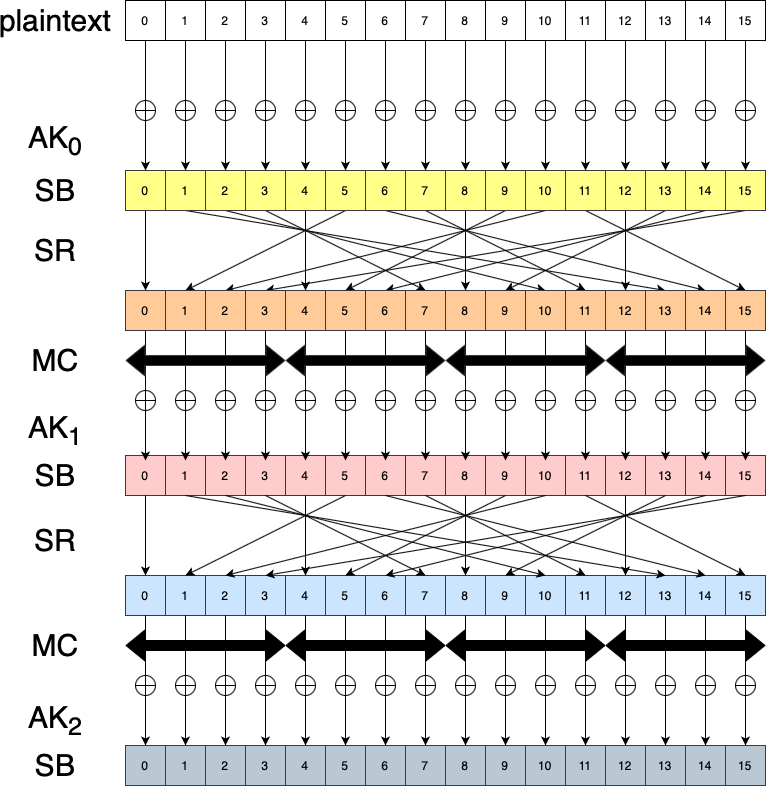
\includegraphics[scale=0.4]{AES-diffusion.drawio.png}
    \caption{Illustrating the AES round transformations. The $X$ symbol is omitted for simplicity. White refers to plaintext, yellow to $x^{1, SB}$, orange to $x^{1, SR}$, pink to $x^{2, SB}$, blue to $x^{2, SR}$ and grey to $x^{2, SB}$.}
    \label{fig:aes-diff}
\end{figure}

\section{Conclusions}
In this Chapter, we analyzed the AES cipher with respect to the complete diffusion property, and showed that complete plaintext diffusion is achieved by the end of the second iteration, for all parameter sets. We also showed that complete key diffusion is achieved by the end of the second iteration for a key size of 128 bits and, for the key sizes 192 and 256, it is achieved by the end of the third iteration. More about the design of AES can be found in \cite{Rijndael}.

From the conducted analysis, the role of each AES component towards achieving complete plaintext and key diffusion is clear. \texttt{SubBytes} ensures diffusion on the bit level, since all the other steps have bytes as their basic unit. \texttt{MixColumns} and \texttt{ShiftRows}, together, ensure that complete diffusion is achieved by the second round of the cipher. Without \texttt{MixColumns}, the elements within each AES state column would not be diffused. Without \texttt{ShiftRows}, elements across different columns would not spread their influence to the state. Therefore, the joint usage of the matrix and the byte permutation is extremely relevant. And, finally, without \texttt{AddRoundKey}, the key would not be diffused.

\bibliographystyle{plain}
\bibliography{refs}
\end{document}
